\documentclass[11pt,a4paper]{article}
\usepackage[utf8]{inputenc}
\usepackage[T1]{fontenc}
\usepackage[spanish,es-nodecimaldot]{babel}
\usepackage{geometry}
\usepackage{booktabs}
\usepackage{xcolor}
\usepackage{hyperref}
\usepackage{array}
\usepackage{graphicx}
\usepackage{float}
\geometry{margin=2.2cm}
\hypersetup{colorlinks=true,linkcolor=blue,urlcolor=blue}

\title{Informe de Hallazgos de Datos\\TechLogistics S.A.S.}
\author{Análisis de EDA, transformación y visualización}
\date{\today}

\begin{document}
\maketitle

\section*{Resumen ejecutivo}
El análisis se realizó sobre la fuente de verdad materializada en
\texttt{data/processed/truth\_dataset.csv}. Se conservaron las ventas cuyos SKU no
aparecen en el maestro de inventario, etiquetándolas como ventas fantasma. Las
transacciones con cantidad no positiva o fecha futura se excluyeron del análisis
operativo, pero se conservaron en los archivos de excluidos.

Los ingresos analizados ascienden a USD 74.572.403,78 y el margen estimado a
USD 14.203.237,50 (19,05\%). El hallazgo de mayor riesgo financiero es que
USD 12.976.848,54 corresponden a ventas sin SKU catalogado, equivalentes al
17,40\% del ingreso total.

\section{Fuga de capital y rentabilidad}
Se localizaron 3.206 registros con margen transaccional negativo, cuyo margen
acumulado es de USD -11.544.543,91. Los SKU con mayor pérdida acumulada son:

\begin{table}[h]
\centering
\caption{Principales SKU con margen acumulado negativo}
\begin{tabular}{lrrr}
\toprule
SKU & Margen (USD) & Ingreso (USD) & Unidades \\
\midrule
PROD-2858 & -57.239,40 & 57.178,37 & 91 \\
PROD-2609 & -49.019,78 & 52.459,07 & 86 \\
PROD-3432 & -43.128,64 & 87.840,68 & 88 \\
PROD-2295 & -41.711,63 & 49.559,00 & 62 \\
PROD-2283 & -39.108,02 & 33.138,42 & 50 \\
\bottomrule
\end{tabular}
\end{table}

El canal Online concentra 770 registros negativos, con pérdida acumulada de
USD -2.784.185,83. Entre sus SKU críticos están PROD-3284 (USD -20.780,68),
PROD-1036 (USD -20.691,23), PROD-2288 (USD -20.055,82) y PROD-1560
(USD -19.423,82).

\textbf{Conclusión gerencial:} no es una pérdida aceptable por volumen. El
volumen es precisamente una señal de que el precio final, el costo unitario o
el costo de envío están mal configurados. La prioridad es congelar promociones
de estos SKU en Online y revisar precio mínimo, descuentos y costo logístico.

\begin{figure}[H]
\centering
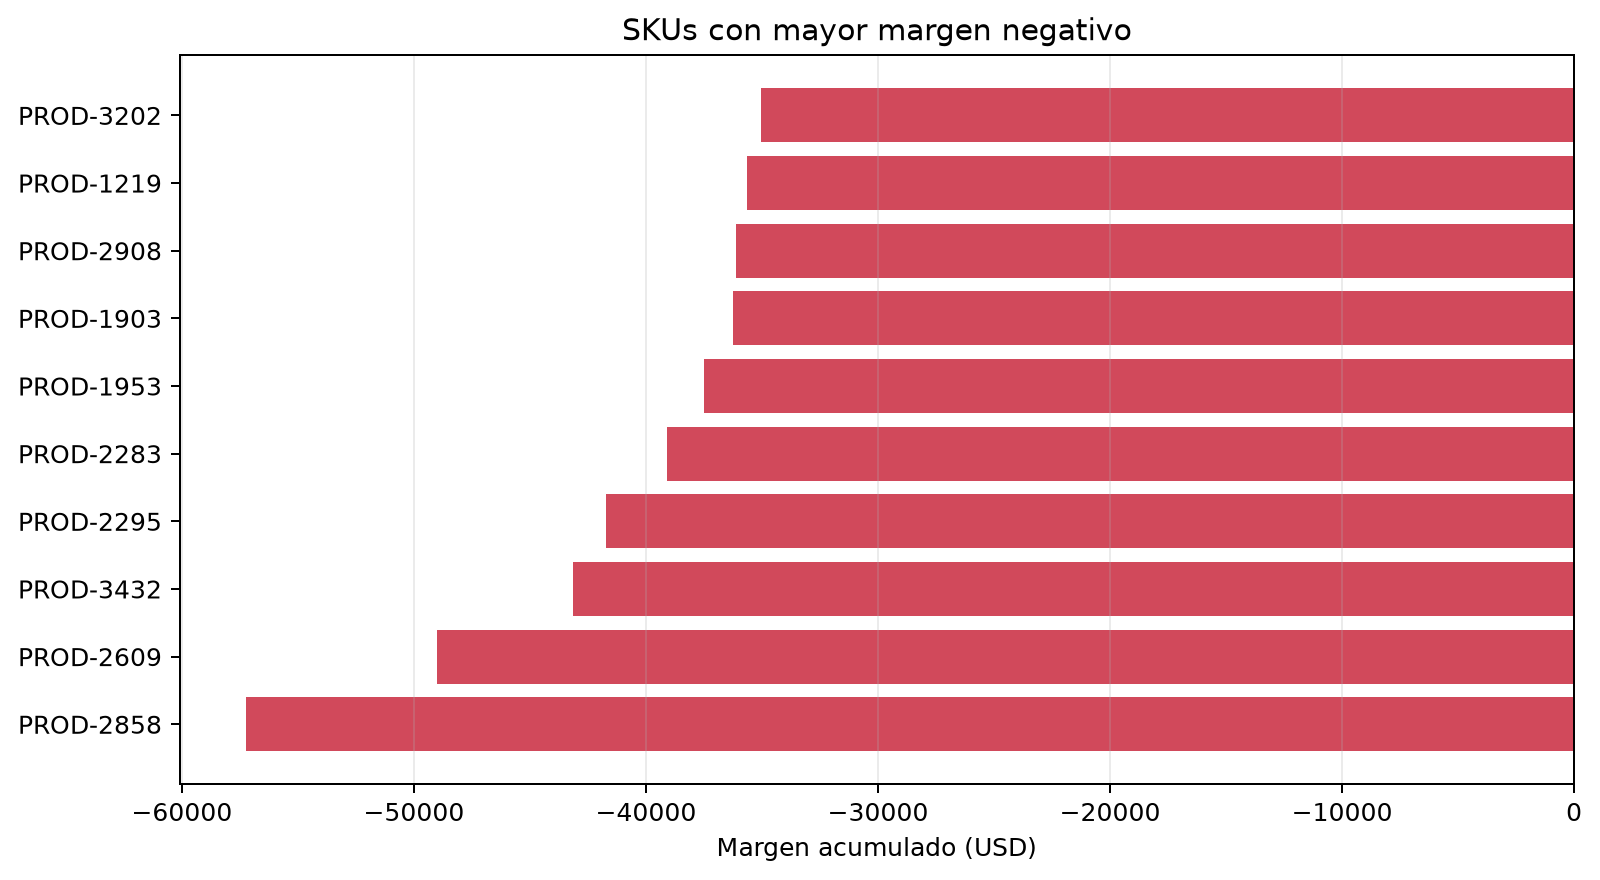
\includegraphics[width=0.9\textwidth]{tex_figures/01_margen_negativo.png}
\caption{Punto 1: SKUs con mayor margen negativo.}
\end{figure}

\section{Crisis logística y cuellos de botella}
La correlación global dentro de cada ciudad entre tiempo de entrega y NPS es
débile: el valor absoluto máximo observado es aproximadamente 0,05 en
Barranquilla. Por ello, el dataset no permite afirmar una relación lineal fuerte;
sin embargo, sí permite localizar concentraciones de insatisfacción.

\begin{table}[h]
\centering
\caption{Ciudades con peor señal de servicio}
\begin{tabular}{lrrr}
\toprule
Ciudad & Entrega promedio (días) & NPS promedio & Correlación \\
\midrule
Barranquilla & 15,28 & -2,95 & 0,052 \\
Ventas\_Web & 14,96 & -3,28 & 0,039 \\
Medellín & 15,21 & 0,10 & 0,011 \\
\bottomrule
\end{tabular}
\end{table}

Por bodega, NORTE presenta el peor NPS promedio (-2,73), seguido por
ZONA\_FRANCA (-0,46). La combinación más crítica por NPS es Bogotá--
ZONA\_FRANCA, con NPS -10,97 y 14,60 días de entrega promedio. Barranquilla--
NORTE también es crítica: NPS -8,90, 15,14 días y 20,45\% de tickets.

\textbf{Decisión:} NORTE requiere el cambio o auditoría inmediata del operador,
con foco inicial en Barranquilla. Bogotá--ZONA\_FRANCA debe permanecer como
segundo frente de intervención. La recomendación debe validarse con SLA,
transportista y tamaño de muestra antes de terminar el contrato, porque la
correlación simple por ciudad es débil.

\begin{figure}[H]
\centering
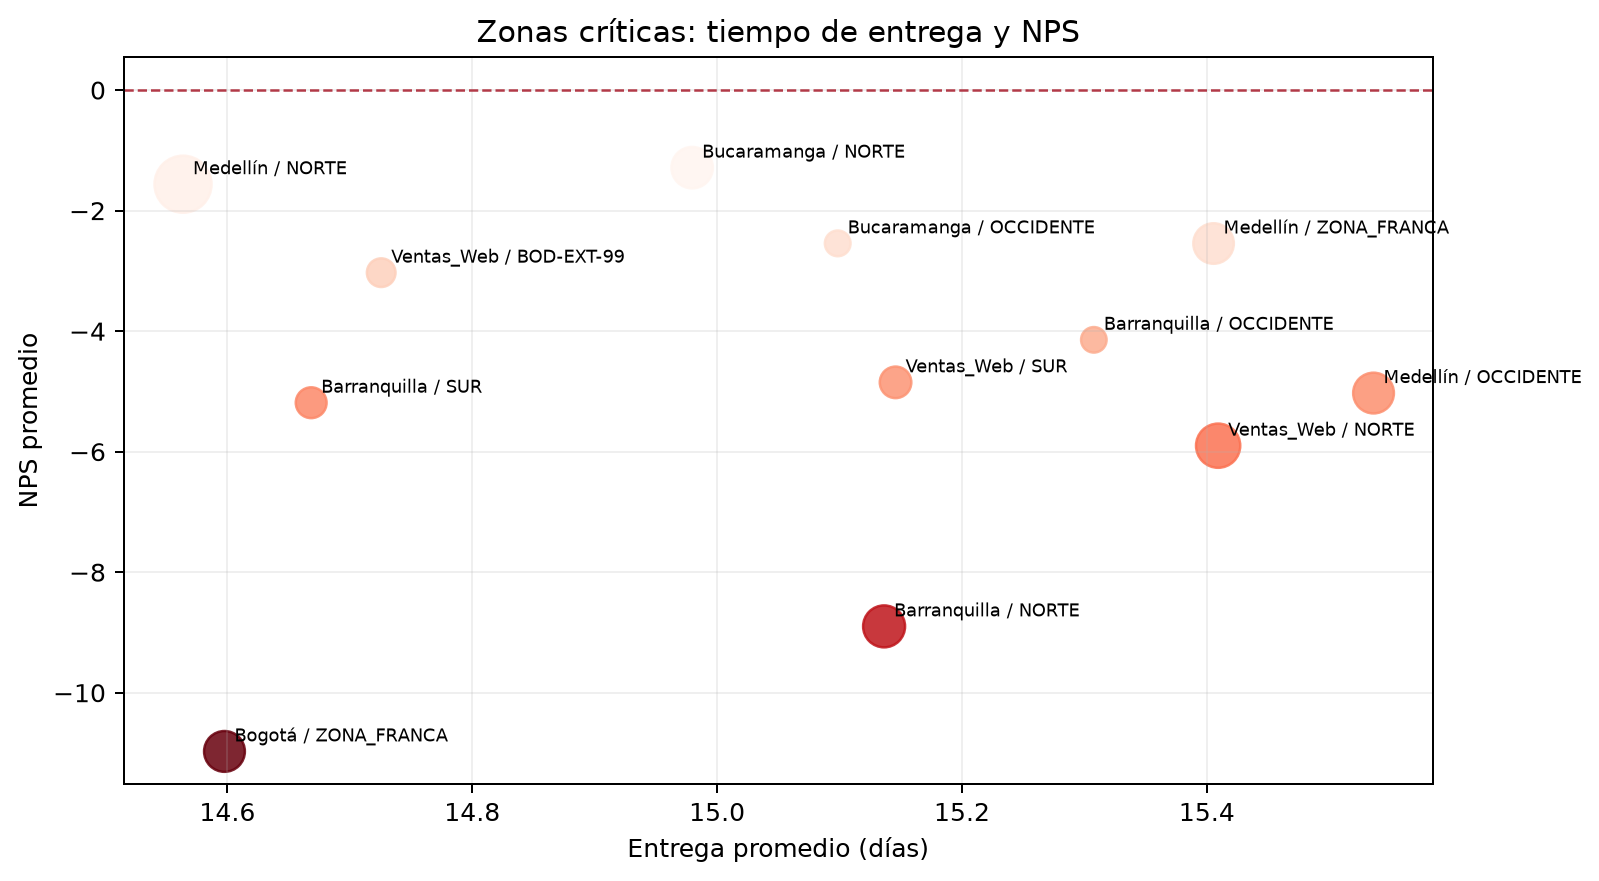
\includegraphics[width=0.9\textwidth]{tex_figures/02_crisis_logistica.png}
\caption{Punto 2: zonas ciudad--bodega con menor NPS y mayor presión logística.}
\end{figure}

\section{Análisis de la venta invisible}
El left join identificó 1.728 transacciones cuyo SKU no aparece en el inventario
oficial. Estas ventas generaron USD 12.976.848,54, que representan:

\[
\frac{12.976.848,54}{74.572.403,78}\times 100 = \mathbf{17,40\%}
\]

del ingreso total analizado. El ingreso se conserva para trazabilidad, pero el
margen de estas ventas no debe interpretarse como confiable porque no existe un
costo unitario oficial asociado.

\textbf{Conclusión gerencial:} la venta invisible es un riesgo de control de
inventario y de reconocimiento de rentabilidad, no una simple anomalía técnica.
Debe cerrarse la brecha entre catálogo, ERP y canales de venta antes de escalar
la operación.

\begin{figure}[H]
\centering
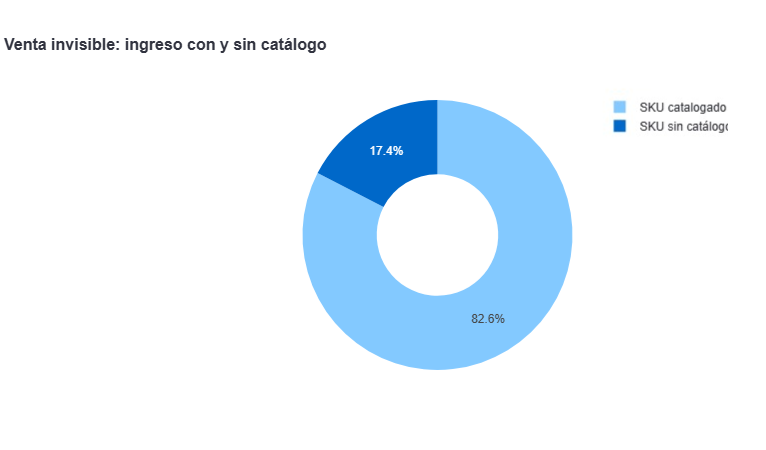
\includegraphics[width=0.35\textwidth]{tex_figures/03_venta_invisible.png}
\caption{Punto 3: ingreso correspondiente a SKU sin catálogo oficial.}
\end{figure}

\section{Diagnóstico de fidelidad}
Sí existe una categoría con alta disponibilidad y sentimiento negativo:
Smartphones tiene stock promedio de 1.017,14 unidades y NPS promedio de -4,82.
También ``Sin categoría'' presenta NPS negativo (-3,13), aunque su problema
principal es de calidad de catálogo.

\begin{figure}[H]
\centering
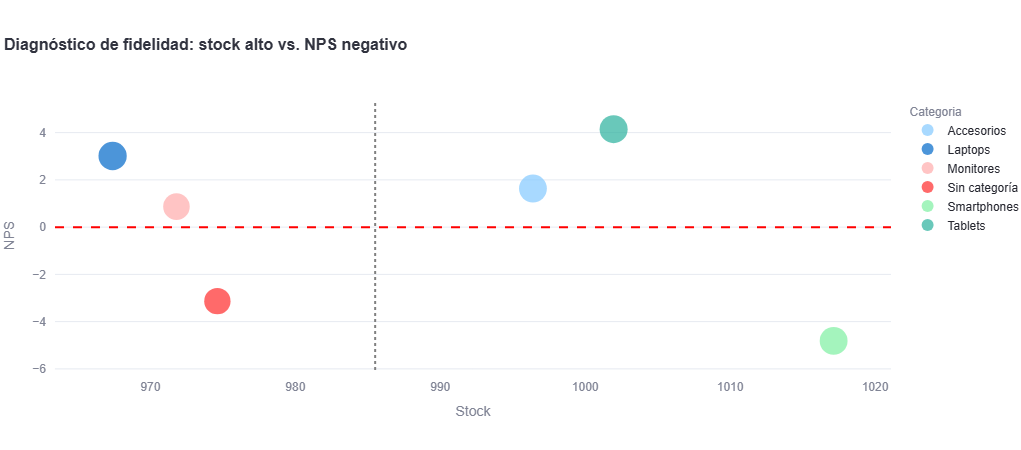
\includegraphics[width=0.9\textwidth]{tex_figures/04_fidelidad.png}
\caption{Punto 4: stock promedio frente a NPS por categoría.}
\end{figure}

\begin{table}[h]
\centering
\caption{Disponibilidad y sentimiento por categoría}
\begin{tabular}{lrrr}
\toprule
Categoría & Stock promedio & NPS promedio & Rating producto \\
\midrule
Smartphones & 1.017,14 & -4,82 & 3,01 \\
Sin categoría & 974,62 & -3,13 & 3,03 \\
Monitores & 971,80 & 0,87 & 2,96 \\
Tablets & 1.001,96 & 4,15 & 3,00 \\
\bottomrule
\end{tabular}
\end{table}

La evidencia apunta más a una combinación de experiencia deficiente y
sobrecosto que a una falla pura de calidad: el rating de producto de Smartphones
es cercano a 3/5, el rating logístico también ronda 3/5 y existe una tasa de
tickets de 15,41\%. La disponibilidad alta no está convirtiéndose en satisfacción;
se debe revisar precio percibido, calidad del producto y promesa de entrega.

\section{Riesgo operativo y bodegas a ciegas}
La antigüedad promedio de la última revisión supera 500 días en todas las
bodegas. Las mayores antigüedades son BOD-EXT-99 (530,57 días), OCCIDENTE
(530,37 días) y ZONA\_FRANCA (522,31 días).

\begin{table}[h]
\centering
\caption{Antigüedad de inventario y soporte}
\begin{tabular}{lrrr}
\toprule
Bodega & Días desde revisión & Tickets (\%) & NPS \\
\midrule
BOD-EXT-99 & 530,57 & 14,11 & 2,96 \\
OCCIDENTE & 530,37 & 16,75 & 1,87 \\
ZONA\_FRANCA & 522,31 & 14,89 & -0,46 \\
NORTE & 519,78 & 15,38 & -2,73 \\
SUR & 504,44 & 14,70 & 0,93 \\
\bottomrule
\end{tabular}
\end{table}

La correlación individual entre días desde revisión y tickets es prácticamente
nula (0,008), por lo que no se debe atribuir causalidad directa. No obstante,
NORTE combina inventario muy antiguo con el peor NPS y ZONA\_FRANCA combina
antigüedad alta con NPS negativo. Estas bodegas operan ``a ciegas'' en términos
de actualización del stock, y la consecuencia observable es menor satisfacción,
especialmente en las rutas críticas identificadas.

\begin{figure}[H]
\centering
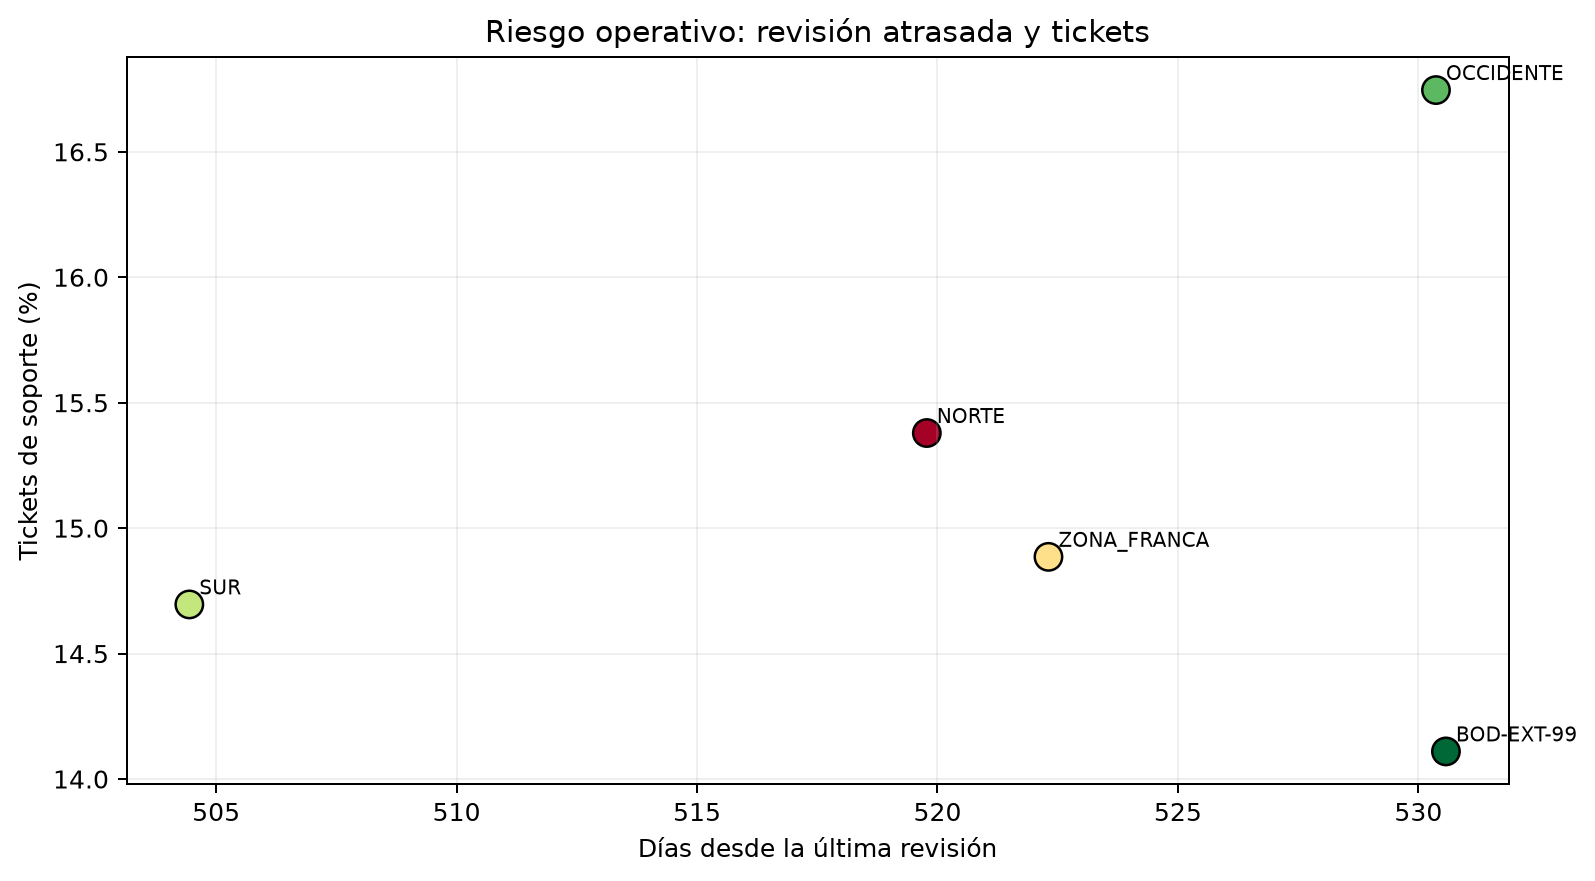
\includegraphics[width=0.9\textwidth]{tex_figures/05_riesgo_operativo.png}
\caption{Punto 5: antigüedad de revisión frente a tickets por bodega.}
\end{figure}

\section*{Plan de acción priorizado}
\begin{enumerate}
  \item \textbf{Alta:} congelar temporalmente SKU Online con margen negativo y conciliar las 1.728 ventas fantasma con el catálogo oficial.
  \item \textbf{Media:} auditar o cambiar el operador asociado a NORTE, comenzando por Barranquilla, y establecer un SLA de entrega medido contra la brecha de lead time.
  \item \textbf{Baja:} programar conteos físicos en BOD-EXT-99, OCCIDENTE, ZONA\_FRANCA y NORTE; activar alertas de stock alto, NPS negativo y tickets.
\end{enumerate}

\end{document}
